\documentclass{beamer}
\usetheme{boadilla}
%\usepackage[scale]{helvet}
\usepackage{etex}
\usepackage{helvet}
\usepackage{translator}

\usepackage[all]{xy}
\usepackage{color}
\usepackage{booktabs}
\usepackage{amsmath,amsthm,amssymb}

\usepackage{fancybox}
\usepackage{comment}
\usepackage{array}
\usepackage{multicol}
\usepackage{multirow}
\usepackage[export]{adjustbox} %for alignment

%% I like helvetica, but here are some other font options
% \usepackage{libertine}
%\usepackage{xunicode}
%\usepackage{xltxtra}
%\usepackage{fontspec}
%\setmainfont{Minion Pro}
%\xyoption{color}
%\xyoption{frame}
%\UseCrayolaColors


\newcommand{\be}{\mathbf{e}}

\newcommand{\bC}{\mathbf{C}}
\newcommand{\bD}{\mathbf{D}}
\newcommand{\bI}{\mathbf{I}}
\newcommand{\bK}{\mathbf{K}}
\newcommand{\bS}{\mathbf{S}}
\newcommand{\bU}{\mathbf{U}}
\newcommand{\bW}{\mathbf{W}}
\newcommand{\bX}{\mathbf{X}}
\newcommand{\bx}{\mathbf{x}}
\newcommand{\bY}{\mathbf{Y}}
\newcommand{\bZ}{\mathbf{Z}}

\newcommand{\bmu}{\boldsymbol\mu}

\newcommand{\bSigma}{\boldsymbol\Sigma}
\newcommand{\bzero}{\mathbf{0}}
\newcommand{\bone}{\mathbf{1}}

\setbeamertemplate{footline}{
\leavevmode%
\hbox{%
\begin{beamercolorbox}[wd=.15\paperwidth,ht=2.25ex,dp=1ex,center]{author in head/foot}%
    \usebeamerfont{title in head/foot}Boca
\end{beamercolorbox}%
\begin{beamercolorbox}[wd=.6\paperwidth,ht=2.25ex,dp=1ex,center]{title in head/foot}%
    \usebeamerfont{title in head/foot}\insertshorttitle
\end{beamercolorbox}%
\begin{beamercolorbox}[wd=.25\paperwidth,ht=2.25ex,dp=1ex,right]{date in head/foot}%
    \usebeamerfont{date in head/foot}\insertshortdate{}\hspace*{2em}
    \insertframenumber{} / \inserttotalframenumber\hspace*{2ex} 
\end{beamercolorbox}}%
\vskip0pt%
}
\makeatother

\setbeamertemplate{navigation symbols}{}%remove navigation symbols


\title[High-dimensional data]{High-dimensional data visualization \& analysis in R}
\author{Simina Boca, Matt McCoy}
\date{October 24, 2018}
\institute{Innovation Center for Biomedical Informatics, Georgetown University Medical Center} \vspace{1.5cm}

\begin{document}

\begin{frame}[plain,t,noframenumbering]
\titlepage
\end{frame}

%%%%%%%%%%%%%%%%%%%%%%%%%
%%%%%%%%%%%%%%%%%%%%%%%%%
%%%%%%%%%%%%%%%%%%%%%%%%%

\begin{frame}
\frametitle{Process of data analysis}

\begin{itemize}
\item Data analysis is a multi-stage process!
\item Generally process goes from experimental design to inference.
\begin{itemize}
\item Includes data cleaning, exploratory data analysis prior to modelling.
\item Sometimes the pre-inference steps are called ``data janitorial services" but they are where I spend most
of my time and essential to really understanding what is going on!
\end{itemize}
\end{itemize}

\vspace{0.4cm}

Leek and Peng, \textit{Nature}, 2015

\end{frame}

%%%%%%%%%%%%%%%%%%%%%%%%%
%%%%%%%%%%%%%%%%%%%%%%%%%
%%%%%%%%%%%%%%%%%%%%%%%%%

\begin{frame}
\frametitle{High-dimensional data}

\begin{itemize}
\item Generally defined as scenarios where the number of features being measured (p) is larger than the number of samples (n).
\item p can often be very large (hundreds, thousands, millions!)
\item Makes it harder to visualize and analyze the data
\item Examples?

\end{itemize}

\end{frame}

%%%%%%%%%%%%%%%%%%%%%%%%%
%%%%%%%%%%%%%%%%%%%%%%%%%
%%%%%%%%%%%%%%%%%%%%%%%%%

\begin{frame}
\frametitle{High-dimensional data}

\begin{itemize}
\item Generally defined as scenarios where the number of features being measured (p) is larger than the number of samples (n).
\item p can often very large (hundreds, thousands, millions!)
\item Makes it harder to visualize and analyze the data
\item Examples? {\color{orange}All omics datasets, imaging data, wearable technology and other time-series data etc}

\end{itemize}

\end{frame}

%%%%%%%%%%%%%%%%%%%%%%%%%
%%%%%%%%%%%%%%%%%%%%%%%%%
%%%%%%%%%%%%%%%%%%%%%%%%%

\begin{frame}
\frametitle{Is it better to have more data?}

\end{frame}

%%%%%%%%%%%%%%%%%%%%%%%%%
%%%%%%%%%%%%%%%%%%%%%%%%%
%%%%%%%%%%%%%%%%%%%%%%%%%

\begin{frame}
\frametitle{Is it better to have more data?}

\begin{itemize}
\item It can be, but it also depends on context!
\item Need to keep in mind all the ideas used for ``small data" when analyzing ``big data" as well as additional
issues that may arise.
\item The study/context in which the data were collected is key, otherwise you may answer the wrong question!
\end{itemize}

\end{frame}

%%%%%%%%%%%%%%%%%%%%%%%%%
%%%%%%%%%%%%%%%%%%%%%%%%%
%%%%%%%%%%%%%%%%%%%%%%%%%

\begin{frame}
\frametitle{Exploratory data analysis (EDA)}

\begin{itemize}
\item Look at dataset in several different ways before starting to model!
\begin{itemize}
\item Immediately starting to model or perform t-tests etc is almost always a bad idea.
\end{itemize}
\item EDA is essential for any data analysis!
\item Consider a combination of:
\begin{itemize}
\item {\color{orange}Tables}: Number of missing or unusual values, ranges, quantiles
\item {\color{orange}Graphs}: Boxplots, scatterplots, clustering
\end{itemize}

\end{itemize}

\end{frame}

%%%%%%%%%%%%%%%%%%%%%%%%%
%%%%%%%%%%%%%%%%%%%%%%%%%
%%%%%%%%%%%%%%%%%%%%%%%%%

\begin{frame}
\frametitle{Exploratory data analysis (EDA)}

\begin{itemize}
\item For high-dimensional data, typically  have demographic/clinical characteristics for
individuals or samples along with omics or imaging data - need to do EDA for both!
\begin{itemize}
\item {\color{orange}In our example, have disease status (Duchenne muscular dystrophy vs healthy), age, and study site, along with metabolite measurements.}
\end{itemize}
\item Tips at \url{https://github.com/SiminaB/Mentoring/blob/master/Omics_exploratory_analysis_checklist.md}
and \url{https://leanpub.com/exdata} (book by Roger Peng - can download for free!)
\end{itemize}

\end{frame}

%%%%%%%%%%%%%%%%%%%%%%%%%
%%%%%%%%%%%%%%%%%%%%%%%%%
%%%%%%%%%%%%%%%%%%%%%%%%%

\begin{frame}
\frametitle{Visualizing high-dimensional data}

\begin{itemize}
\item {\color{orange}``You have to make big data into small data to visualize it."}[I forget who said this]
\item Can think of your data as an n x p matrix. 
\item Graphs are only in 2D, though can represent additional dimensions using colors, symbols etc.
\item {\color{orange} How can we reduce dimensionality?}
\end{itemize}

\end{frame}

%%%%%%%%%%%%%%%%%%%%%%%%%
%%%%%%%%%%%%%%%%%%%%%%%%%
%%%%%%%%%%%%%%%%%%%%%%%%%

\begin{frame}
\frametitle{Visualizing high-dimensional data}

\begin{itemize}
\item {\color{orange} How can we reduce dimensionality?}
\item One commonly used approach is principal component analysis (PCA), which decomposes the matrix into the directions of 
highest variability that can be expressed as orthogonal linear combinations of the original features.
\begin{itemize}
\item The first principal component (PC) is an n x 1 vector that captures the most variability from the original dataset (among all possible linear combinations), the 2nd PC is an n x 1 vector that captures the most variability orthogonal on the first etc.
\item Often look at the first 2 PCs - in the resulting plot, each point is a sample and the value is a combination of all the features.
\item {\color{orange}Generally helpful to perform PCA on omics dataset, then represent clinical/demographic characteristics via different colors, shapes etc.}
\end{itemize}
\end{itemize}

\end{frame}

%%%%%%%%%%%%%%%%%%%%%%%%%
%%%%%%%%%%%%%%%%%%%%%%%%%
%%%%%%%%%%%%%%%%%%%%%%%%%

\begin{frame}
\frametitle{Why is PCA helpful?}

\begin{itemize}
\item It gives a general idea of overall features of the dataset (can formalize with statistical tests)
\item It can identify outlying samples (which could not be identified looking at thousands or tens of thousand of dimensions!)
\item It can identify potential artifacts or batch effects, like samples processed in different ways
\end{itemize}

\vspace{0.3cm}

Read Leek et al, \textit{Nature Reviews Genetics}, 2010, for more details on batch effects and using PCA or clustering
to detect them.

\end{frame}

%%%%%%%%%%%%%%%%%%%%%%%%%
%%%%%%%%%%%%%%%%%%%%%%%%%
%%%%%%%%%%%%%%%%%%%%%%%%%

\begin{frame}
\frametitle{Performing statistical analysis for high-dimensional data}

\begin{itemize}
\item Many techniques exist, depending on whether the goal is inference or prediction.
\item Will focus on inference here, specifically hypothesis testing: 
{\color{orange}What metabolites are significantly associated with 
Duchenne muscular dystrophy, adjusting for age and study site and allowing for different trends with age in cases
and controls?}
\item Approach is to fit a regression model for each metabolite, then adjust for multiple testing.
\item In the end, get a list of metabolites that should be followed up in future studies.

\end{itemize}

\end{frame}

%%%%%%%%%%%%%%%%%%%%%%%%%
%%%%%%%%%%%%%%%%%%%%%%%%%
%%%%%%%%%%%%%%%%%%%%%%%%%

\begin{frame}
\frametitle{Multiple testing issues}

\begin{itemize}
\item If the null hypothesis (of no difference) holds true when performing a single statistical test,
then a p-value $< 0.05$ will be observed 5\% of the time (over repeated experiments).
\item When performing $m$ statistical tests, even if the null hypotheses are all true, we will expect
$0.05 \times m$ rejections at the $p = 0.05$ level.
\item Can address this in multiple ways, for example by controlling the family-wise error rate (FWER)
via the Bonferroni correction or the false discovery rate (FDR) via the Benjamini-Hochberg (BH) procedure.
\end{itemize}

\end{frame}

%%%%%%%%%%%%%%%%%%%%%%%%%
%%%%%%%%%%%%%%%%%%%%%%%%%
%%%%%%%%%%%%%%%%%%%%%%%%%

\begin{frame}
\frametitle{Reproducibility: An essential component of a data analysis}

\begin{itemize}
\item Reproducibility refers to making the data and code of a project available so that anyone can run the same analysis
and get the same results.
\item When using R, one approach is to use R markdown, which combines text, code, and output.
\item Reproducibility is helpful for the scientific community, but also for yourself.
\end{itemize}

\end{frame}

%%%%%%%%%%%%%%%%%%%%%%%%%
%%%%%%%%%%%%%%%%%%%%%%%%%
%%%%%%%%%%%%%%%%%%%%%%%%%

\begin{frame}
\frametitle{Reproducibility: An essential component of a data analysis}

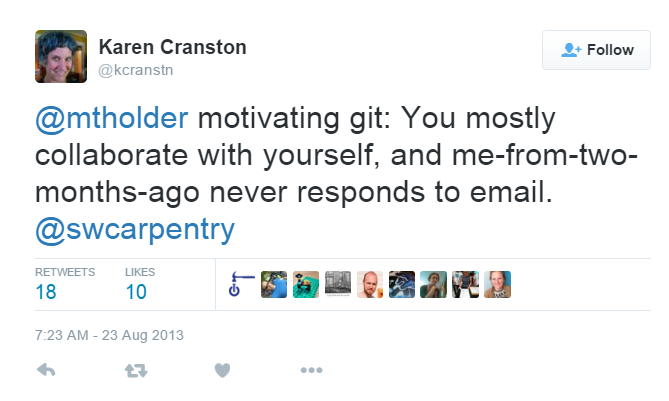
\includegraphics[height=0.72\textheight, center]{reproducibility_tweet.png}

\end{frame}

%%%%%%%%%%%%%%%%%%%%%%%%%
%%%%%%%%%%%%%%%%%%%%%%%%%
%%%%%%%%%%%%%%%%%%%%%%%%%

\end{document}






